A comparison of the average D-h correlation distributions on the new p-Pb data samples with expectations from Monte Carlo simulations (currently Pythia6-Perugia2011, Pythia6-Perugia2010, Pythia6-Perugia0, PYTHIA8; POWHEG+PYTHIA and EPOS 3 will be added if they come in time) is shown in Figure \ref{fig:CfrAverageModel}, after the baseline subtraction (which differs strongly between data and simulations, due to he very different underlying event). The simulations, though being for pp, include the boost of the center-of-mass along the beam axis present in p-Pb collisions and nuclear PDF. The shape of the correlation distributions is well reproduced by all the models, together with their $\pt$ trend and with the evolution of the correlation peaks.

\begin{figure}[!htbp]
\centering
\landscape
{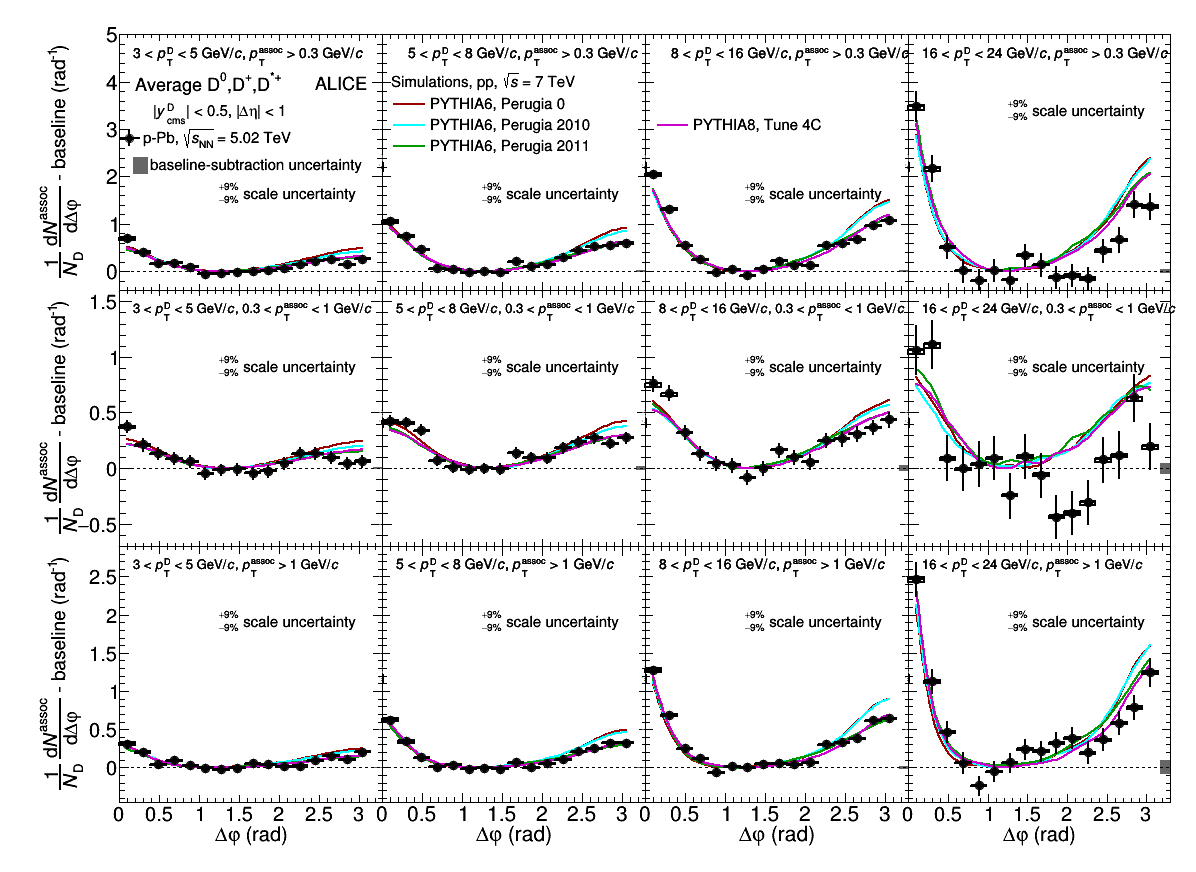
\includegraphics[width=\linewidth]{figures/CfrPPandModels/CorrelationppMC4x6_1New.png}}
{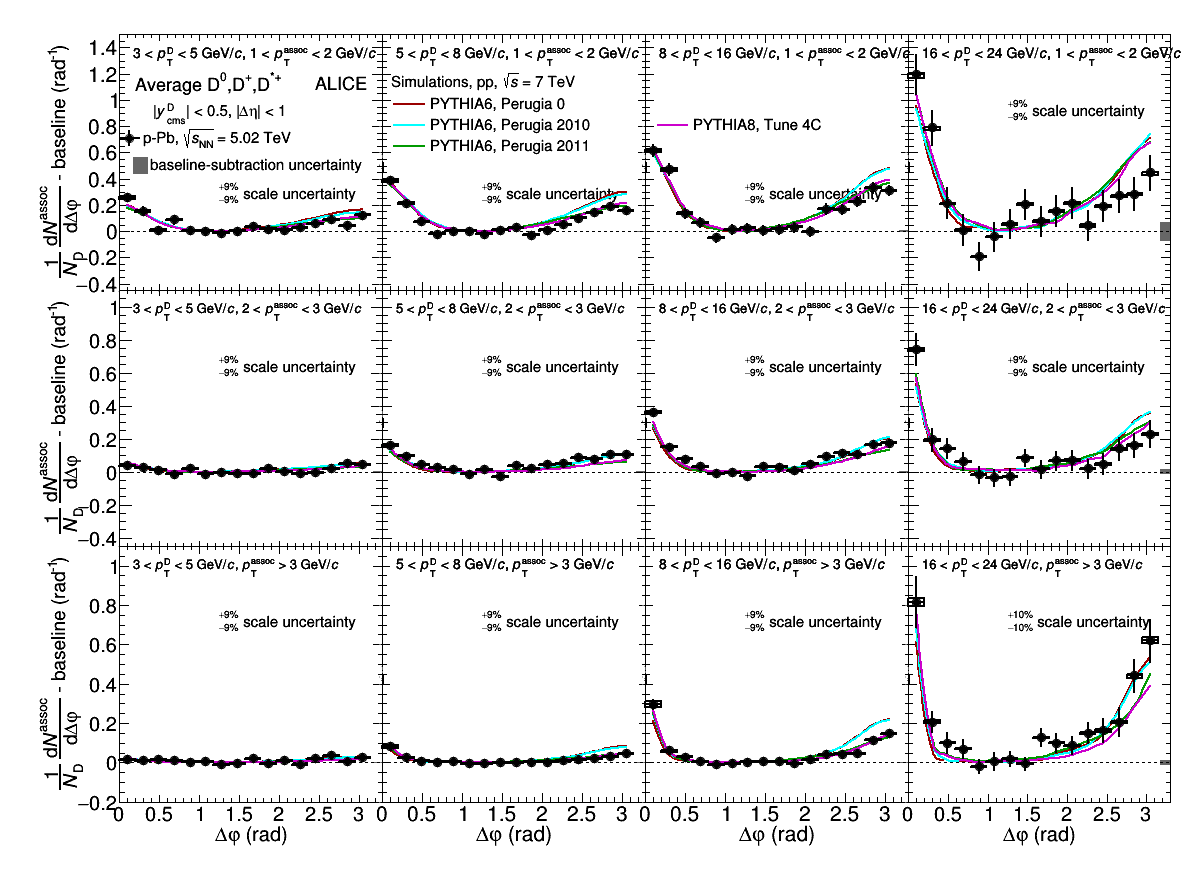
\includegraphics[width=\linewidth]{figures/CfrPPandModels/CorrelationppMC4x6_2New.png}}
\caption{Comparison of p-Pb 2016 average D-h correlation distributions and model expectations, for all the studied kinematic ranges.}
\label{fig:CfrAverageModel}
\end{figure}

Figures \ref{fig:CfrObsModel} and \ref{fig:CfrObsModel2} show the same comparison for the fit observables (peak yields and widths for near-side and away-side, respectively), for all the addressed $\pt$ ranges. 

\begin{figure}[!htbp]
\centering
\landscape
{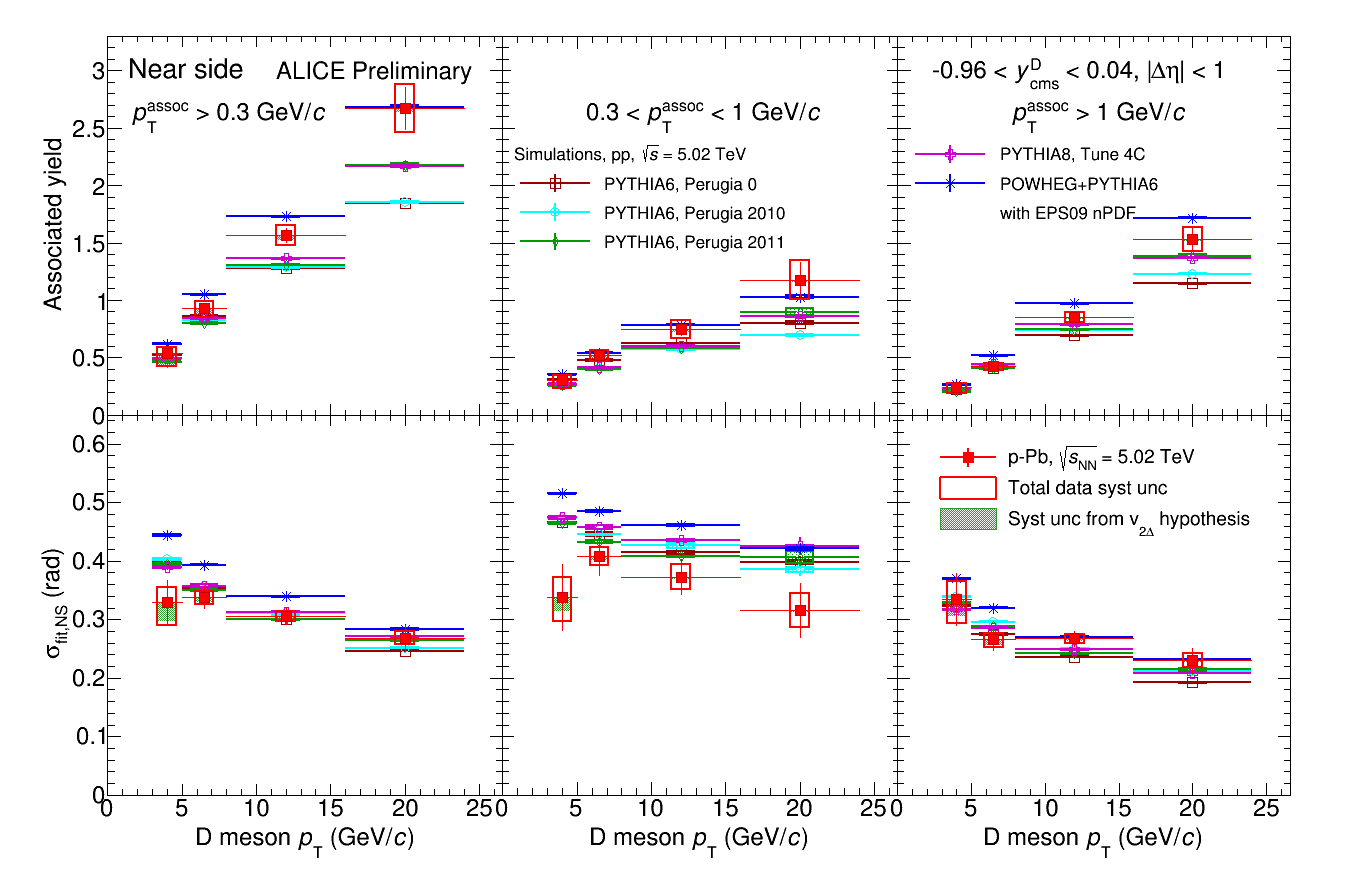
\includegraphics[width=\linewidth]{figures/CfrPPandModels/ComparePPbtoMCFitResults.png}}
{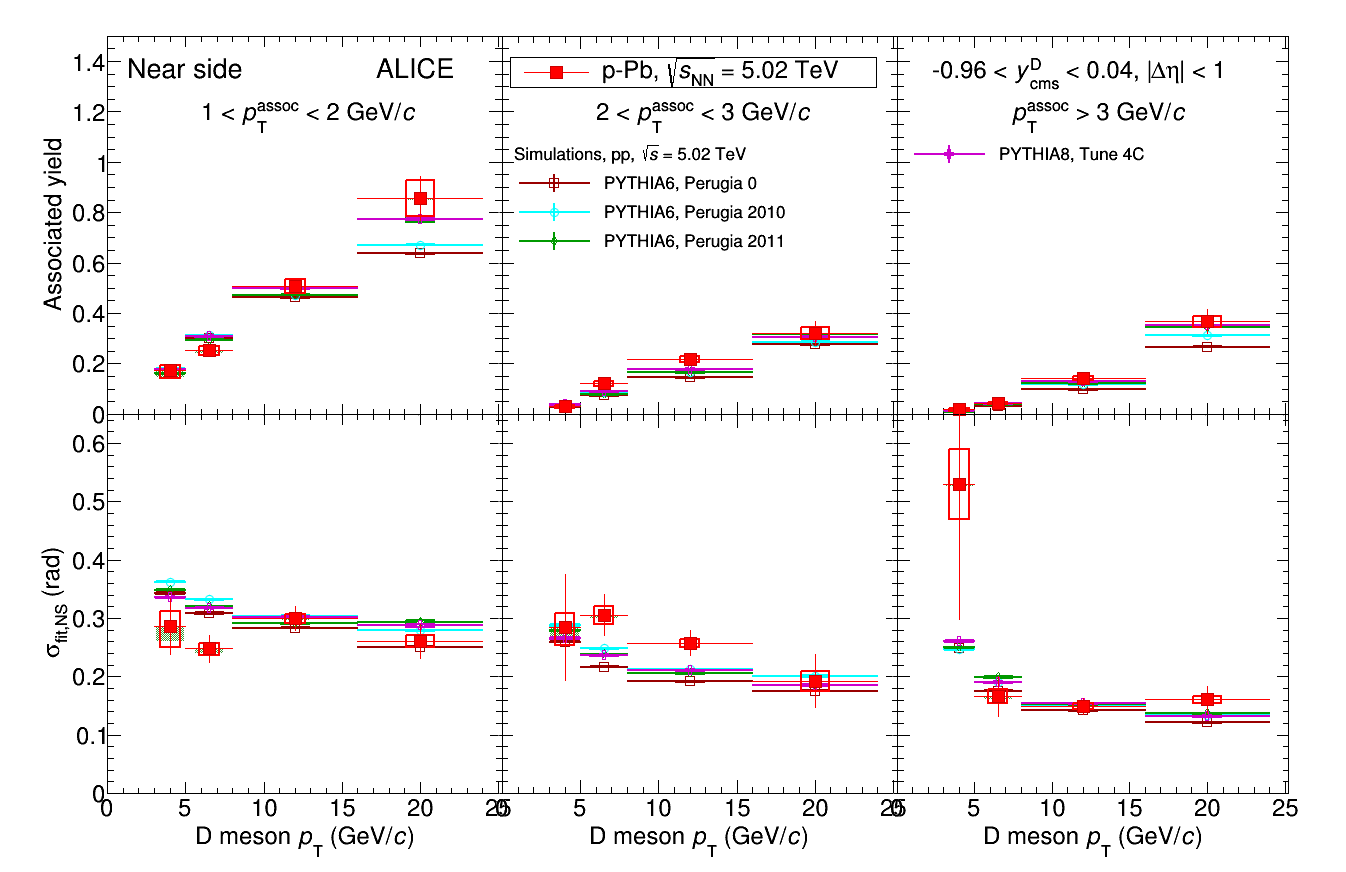
\includegraphics[width=\linewidth]{figures/CfrPPandModels/ComparePPbtoMCFitResults_2.png}}
\caption{Comparison of near-side peak yields and widths from p-Pb 2016 results and model expectations, for all the studied kinematic ranges.}
\label{fig:CfrAverageModel}
\end{figure}
\begin{figure}[!htbp]
\centering
\landscape
{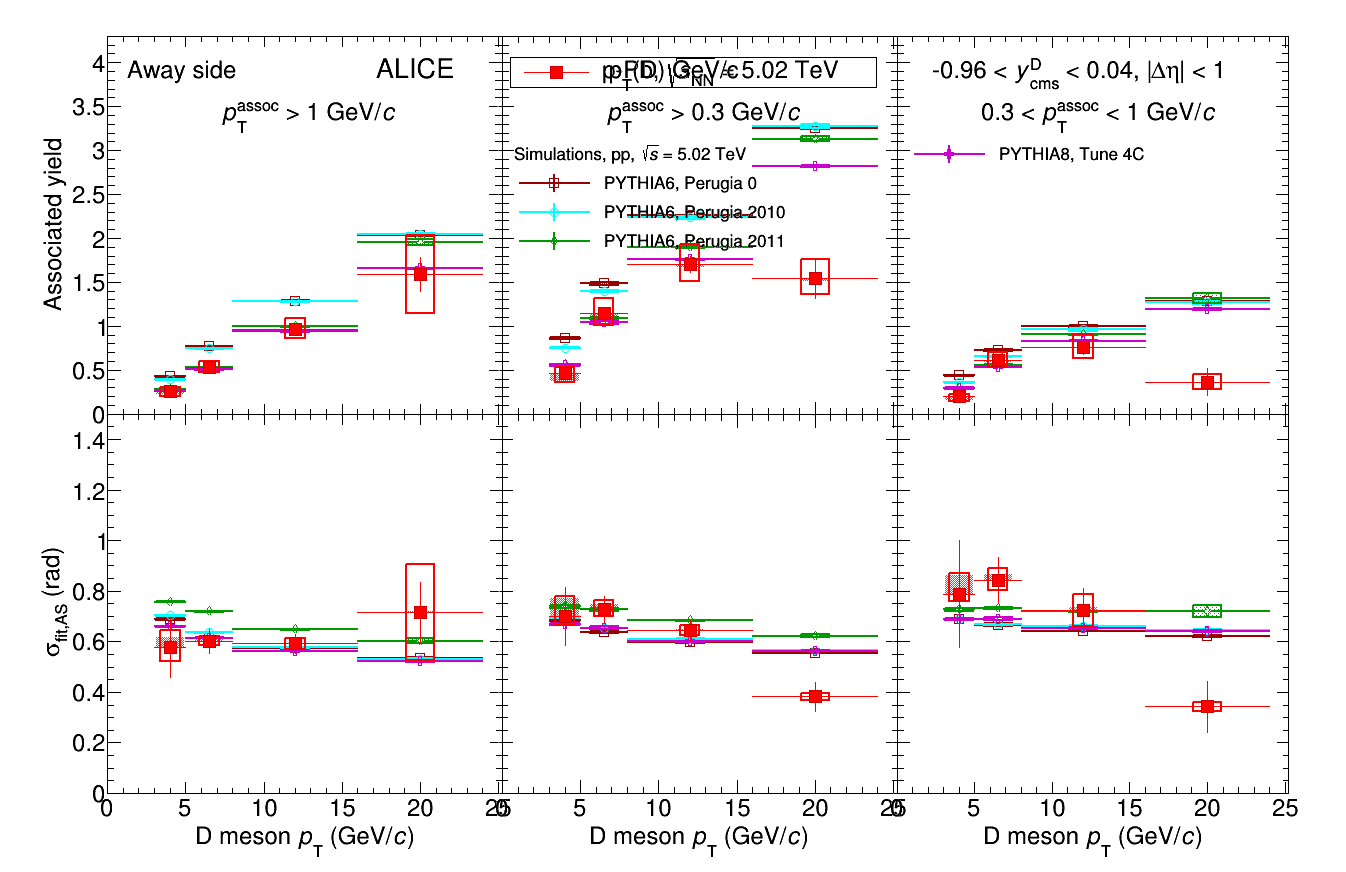
\includegraphics[width=\linewidth]{figures/CfrPPandModels/ComparePPbtoMCFitResultsAS.png}}
{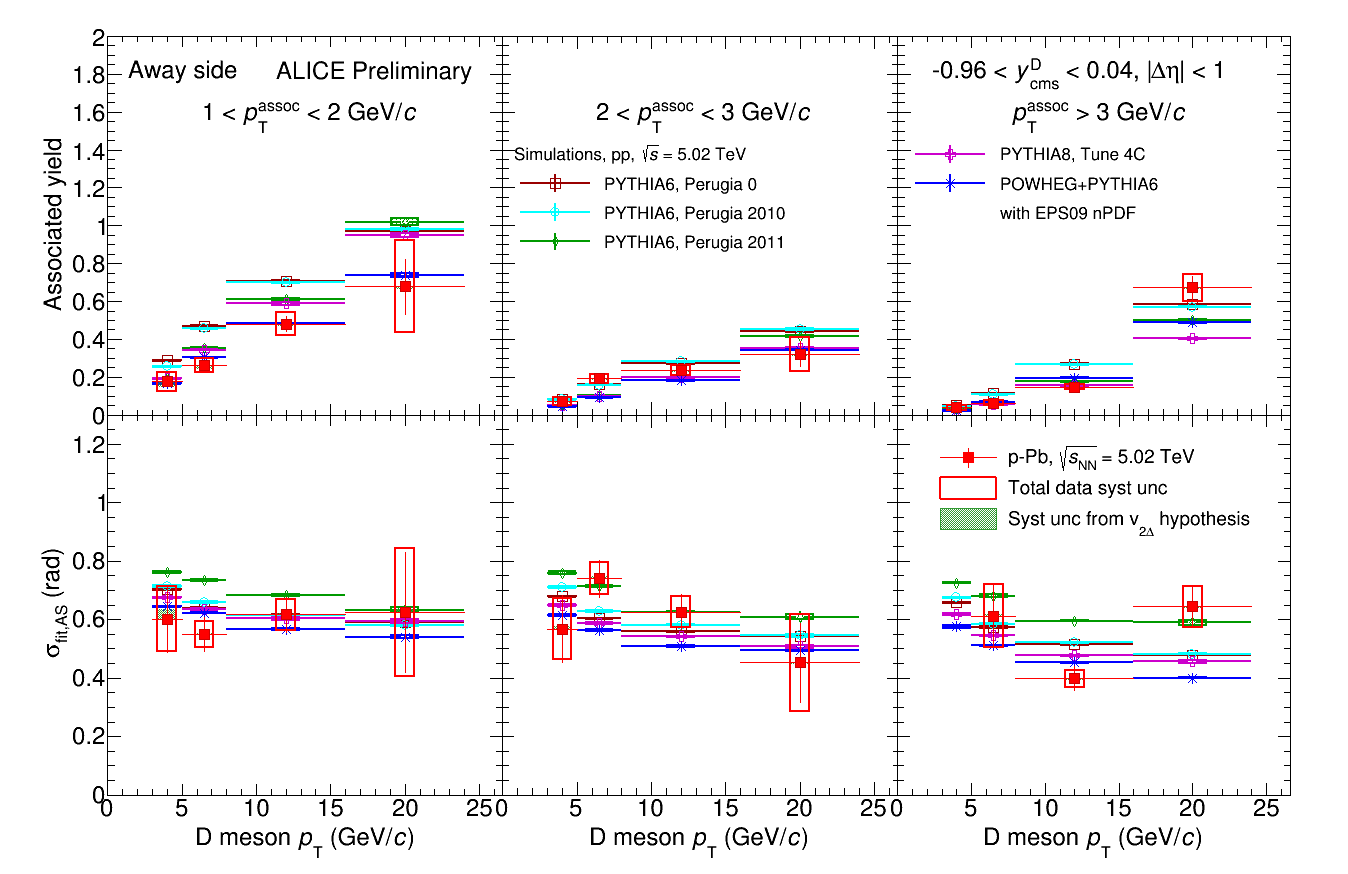
\includegraphics[width=\linewidth]{figures/CfrPPandModels/ComparePPbtoMCFitResultsAS_2.png}}
\caption{Comparison of away-side peak yields and widths from p-Pb 2016 results and model expectations, for all the studied kinematic ranges.}
\label{fig:CfrAverageModel2}
\end{figure}
